% Options for packages loaded elsewhere
\PassOptionsToPackage{unicode}{hyperref}
\PassOptionsToPackage{hyphens}{url}
%
\documentclass[
  english,
  man,floatsintext]{apa6}
\usepackage{lmodern}
\usepackage{amssymb,amsmath}
\usepackage{ifxetex,ifluatex}
\ifnum 0\ifxetex 1\fi\ifluatex 1\fi=0 % if pdftex
  \usepackage[T1]{fontenc}
  \usepackage[utf8]{inputenc}
  \usepackage{textcomp} % provide euro and other symbols
\else % if luatex or xetex
  \usepackage{unicode-math}
  \defaultfontfeatures{Scale=MatchLowercase}
  \defaultfontfeatures[\rmfamily]{Ligatures=TeX,Scale=1}
\fi
% Use upquote if available, for straight quotes in verbatim environments
\IfFileExists{upquote.sty}{\usepackage{upquote}}{}
\IfFileExists{microtype.sty}{% use microtype if available
  \usepackage[]{microtype}
  \UseMicrotypeSet[protrusion]{basicmath} % disable protrusion for tt fonts
}{}
\makeatletter
\@ifundefined{KOMAClassName}{% if non-KOMA class
  \IfFileExists{parskip.sty}{%
    \usepackage{parskip}
  }{% else
    \setlength{\parindent}{0pt}
    \setlength{\parskip}{6pt plus 2pt minus 1pt}}
}{% if KOMA class
  \KOMAoptions{parskip=half}}
\makeatother
\usepackage{xcolor}
\IfFileExists{xurl.sty}{\usepackage{xurl}}{} % add URL line breaks if available
\IfFileExists{bookmark.sty}{\usepackage{bookmark}}{\usepackage{hyperref}}
\hypersetup{
  pdftitle={Using contrastive inferences to learn about new words and categories},
  pdfauthor={Claire Augusta Bergey1 \& Daniel Yurovsky2},
  pdflang={en-EN},
  pdfkeywords={concept learning; contrastive inference; word learning; pragmatics; communication; computational modeling},
  hidelinks,
  pdfcreator={LaTeX via pandoc}}
\urlstyle{same} % disable monospaced font for URLs
\usepackage{graphicx}
\makeatletter
\def\maxwidth{\ifdim\Gin@nat@width>\linewidth\linewidth\else\Gin@nat@width\fi}
\def\maxheight{\ifdim\Gin@nat@height>\textheight\textheight\else\Gin@nat@height\fi}
\makeatother
% Scale images if necessary, so that they will not overflow the page
% margins by default, and it is still possible to overwrite the defaults
% using explicit options in \includegraphics[width, height, ...]{}
\setkeys{Gin}{width=\maxwidth,height=\maxheight,keepaspectratio}
% Set default figure placement to htbp
\makeatletter
\def\fps@figure{htbp}
\makeatother
\setlength{\emergencystretch}{3em} % prevent overfull lines
\providecommand{\tightlist}{%
  \setlength{\itemsep}{0pt}\setlength{\parskip}{0pt}}
\setcounter{secnumdepth}{-\maxdimen} % remove section numbering
% Make \paragraph and \subparagraph free-standing
\ifx\paragraph\undefined\else
  \let\oldparagraph\paragraph
  \renewcommand{\paragraph}[1]{\oldparagraph{#1}\mbox{}}
\fi
\ifx\subparagraph\undefined\else
  \let\oldsubparagraph\subparagraph
  \renewcommand{\subparagraph}[1]{\oldsubparagraph{#1}\mbox{}}
\fi
% Manuscript styling
\usepackage{upgreek}
\captionsetup{font=singlespacing,justification=justified}

% Table formatting
\usepackage{longtable}
\usepackage{lscape}
% \usepackage[counterclockwise]{rotating}   % Landscape page setup for large tables
\usepackage{multirow}		% Table styling
\usepackage{tabularx}		% Control Column width
\usepackage[flushleft]{threeparttable}	% Allows for three part tables with a specified notes section
\usepackage{threeparttablex}            % Lets threeparttable work with longtable

% Create new environments so endfloat can handle them
% \newenvironment{ltable}
%   {\begin{landscape}\begin{center}\begin{threeparttable}}
%   {\end{threeparttable}\end{center}\end{landscape}}
\newenvironment{lltable}{\begin{landscape}\begin{center}\begin{ThreePartTable}}{\end{ThreePartTable}\end{center}\end{landscape}}

% Enables adjusting longtable caption width to table width
% Solution found at http://golatex.de/longtable-mit-caption-so-breit-wie-die-tabelle-t15767.html
\makeatletter
\newcommand\LastLTentrywidth{1em}
\newlength\longtablewidth
\setlength{\longtablewidth}{1in}
\newcommand{\getlongtablewidth}{\begingroup \ifcsname LT@\roman{LT@tables}\endcsname \global\longtablewidth=0pt \renewcommand{\LT@entry}[2]{\global\advance\longtablewidth by ##2\relax\gdef\LastLTentrywidth{##2}}\@nameuse{LT@\roman{LT@tables}} \fi \endgroup}

% \setlength{\parindent}{0.5in}
% \setlength{\parskip}{0pt plus 0pt minus 0pt}

% \usepackage{etoolbox}
\makeatletter
\patchcmd{\HyOrg@maketitle}
  {\section{\normalfont\normalsize\abstractname}}
  {\section*{\normalfont\normalsize\abstractname}}
  {}{\typeout{Failed to patch abstract.}}
\patchcmd{\HyOrg@maketitle}
  {\section{\protect\normalfont{\@title}}}
  {\section*{\protect\normalfont{\@title}}}
  {}{\typeout{Failed to patch title.}}
\makeatother
\shorttitle{Learning from contrastive inference}
\keywords{concept learning; contrastive inference; word learning; pragmatics; communication; computational modeling\newline\indent Word count: 11021}
\usepackage{lineno}

\linenumbers
\usepackage{csquotes}
\ifxetex
  % Load polyglossia as late as possible: uses bidi with RTL langages (e.g. Hebrew, Arabic)
  \usepackage{polyglossia}
  \setmainlanguage[]{english}
\else
  \usepackage[shorthands=off,main=english]{babel}
\fi
\newlength{\cslhangindent}
\setlength{\cslhangindent}{1.5em}
\newenvironment{cslreferences}%
  {\setlength{\parindent}{0pt}%
  \everypar{\setlength{\hangindent}{\cslhangindent}}\ignorespaces}%
  {\par}

\title{Using contrastive inferences to learn about new words and categories}
\author{Claire Augusta Bergey\textsuperscript{1} \& Daniel Yurovsky\textsuperscript{2}}
\date{}


\authornote{

All data and code for analyses are available at \url{https://github.com/cbergey/contrast}.

Correspondence concerning this article should be addressed to Claire Augusta Bergey, 5848 S. University Avenue, Chicago, IL 60637. E-mail: \href{mailto:cbergey@uchicago.edu}{\nolinkurl{cbergey@uchicago.edu}}

}

\affiliation{\vspace{0.5cm}\textsuperscript{1} University of Chicago\\\textsuperscript{2} Carnegie Mellon University}

\abstract{
In the face of unfamiliar language or objects, description is one cue people can use to learn about both. Beyond narrowing potential referents to those that match a descriptor (e.g., ``tall''), people could infer that a described object is one that contrasts with other relevant objects of the same type (e.g., ``the tall cup'' contrasts with another, shorter cup). This contrast may be in relation to other objects present in the environment (this cup is tall among present cups) or to the referent's category (this cup is tall for a cup in general). In three experiments, we investigate whether people use such contrastive inferences from description to learn new word-referent mappings and learn about new categories' feature distributions. People use contrastive inferences to guide their referent choice, though size---and not color---adjectives prompt them to consistently choose the contrastive target over alternatives (Experiment 1). People also use color and size description to infer that a novel object is atypical of its category (Experiments 2 and 3): utterances like ``the blue toma'' prompt people to infer that tomas are \emph{less} likely to be blue in general. However, these two inferences do not trade off substantially: people infer a described referent is atypical even when the descriptor was necessary to establish reference. We model these experiments in the Rational Speech Act (RSA) framework and find that it predicts both of these inferences. Overall, people are able to use contrastive inferences from description to resolve reference and make inferences about a novel object's category, letting them learn more about new things than literal meaning alone allows.
}



\begin{document}
\maketitle

An utterance can say much more about the world than its literal interpretation might suggest. For instance, if you hear a colleague say ``We should hire a female professor,'' you might infer something about the speaker's goals, the makeup of a department, or even the biases of a field---none of which is literally stated. These inferences depend on recognition that a speaker's intended meaning can differ from the literal meaning of their utterance, and the process of deriving this intended meaning is called \emph{pragmatics}. Frameworks for understanding pragmatic inference posit that speakers tend to follow general principles of conversation---for instance, that they tend to be relevant, brief, and otherwise helpfully informative (Clark, 1990; Grice, 1975; Sperber \& Wilson, 1986). When a speaker deviates from these principles, a listener can reason about the alternative utterances the speaker might have said and infer some intended meaning that goes beyond the literal meaning of their utterance.

Pragmatic inference is also a potentially powerful mechanism for learning language. People can learn the meanings of words by tracking statistical properties of their literal meaning alone (Yu \& Smith, 2007), but reasoning about a speaker's intended meaning---and not just the words they say---may support more rapid and accurate learning (Frank, Goodman, \& Tenenbaum, 2009). For example, Akhtar, Carpenter, and Tomasello (1996) showed that young children can infer the meaning of a new word by using the principle that people tend to remark on things that are new and interesting to them. In their study, an experimenter leaves the room and a new toy emerges in her absence; once she comes back, the toy is familiar to the child but not to the experimenter. When she uses a novel name, ``gazzer,'' the child can infer that the word refers to the toy that is novel to the experimenter, and not other toys the experimenter had already seen. Much other work has emphasized that children can use pragmatic principles to infer a word's meaning, as can adults (Baldwin \& Tomasello, 1998; Bohn \& Frank, 2019; Bohn, Tessler, Merrick, \& Frank, 2021, 2022; Frank \& Goodman, 2014; Gelman \& Markman, 1985; Tomasello, 2000).

One potential pragmatic tool for learning about referents is contrastive inference from description. To the extent that communicators strive to be minimal and informative, description should discriminate between the referent and some relevant contrasting set. This contrastive inference is fairly obvious from some types of description, such as some modifying adjunct phrases: ``The door with the lock'' clearly implies a contrasting door without one (Ni, 1996). The degree of contrast implied by more common descriptive forms, such as prenominal adjectives in English, is less clear: speakers do not always use prenominal adjectives minimally, often describing more than is needed to establish reference (Engelhardt, Barış Demiral, \& Ferreira, 2011; Mangold \& Pobel, 1988; Pechmann, 1989). Nevertheless, Sedivy, Tanenhaus, Chambers, and Carlson (1999) showed that people can use these inferences to resolve referential ambiguity in familiar contexts. When asked to ``Pick up the tall cup,'' people directed their attention more quickly to the target when a short cup was present, and did so in the period before they heard the word ``cup.'' Because the speaker would not have needed to specify ``tall'' unless it was informative, listeners were able to use the adjective to direct their attention to a tall object with a shorter counterpart. Subsequent work using similar tasks has corroborated that people can use contrastive inferences to direct their attention among familiar referents and to infer which referents a speaker can see (Aparicio, Xiang, \& Kennedy, 2016; Jara-Ettinger \& Rubio-Fernandez, 2021; Ryskin, Kurumada, \& Brown-Schmidt, 2019; Sedivy, 2003).

But what if you didn't know the meaning of the key words in someone's utterance---could you use the same kind of contrastive inferences to learn about new words and categories? Suppose a friend asks you to ``Pass the tall dax.'' Intuitively, your friend must have said the word ``tall'' for a reason. One possibility is that your friend wants to distinguish the dax they want from another dax they do not. In this case, you might look around the room for two similar things that vary in height, and hand the taller one to them. If, alternatively, you only see one object around whose name you don't know, you might draw a different inference: this dax might be a particularly tall dax. In this case, you might think your friend used the word ``tall'' for a different reason---not to distinguish the dax they want from other daxes around you, but to distinguish the dax they want from other daxes in the world. This would be consistent with data from production studies, in which people tend to describe atypical features more than they describe typical ones (Mitchell, Reiter, \& Deemter, 2013; Rubio-Fernández, 2016; Westerbeek, Koolen, \& Maes, 2015). For instance, people almost always say ``blue banana'' to refer to a blue banana, but almost never say ``yellow banana'' to refer to a yellow one.

In each of these cases, you would have used a pragmatic inference to learn something new. In the second case, you would have learned the name for a novel category ``dax,'' and also something about the typical of size of daxes: most of them are shorter than the one you saw. In the first case, you would have resolved the referential ambiguity in the speaker's utterance. But would you have learned something about the typical size of daxes as well, beyond the daxes you observed? One possibility is that you would not: You can explain your friend's use of ``tall'' as being motivated by the need to distinguish between the two daxes in the room, and thus you should infer nothing about the other daxes in the world. If reference is the primary motivator of speakers' word choice, as implicitly assumed in much research (e.g., Pechmann, 1989; Arts, Maes, Noordman, \& Jansen, 2011; Engelhardt et al., 2011), then people should draw no further inferences once the need for referential disambiguation can explain away a descriptor like ``tall.'' On this \emph{reference-first view}, establishing reference has priority in understanding the utterance, and any further inferences are blocked if the utterance is minimally informative with respect to reference. If, on the other hand, pragmatic reasoning weighs multiple goals simultaneously---here, reference and conveying typicality---people may integrate typicality as just one factor the speaker considers in using description. On this \emph{probabilistic weighing view}, people can use description to make graded inferences about the referent's identity and about its category's features, and the fact that an adjective would have helped identify the referent does not completely block an inference about atypicality.

In this paper, we present a series of experiments that test two ways in which people could use pragmatic inference to learn about novel categories. First, we examine whether listeners use contrastive inference to resolve referential ambiguity. In a reference game, participants saw groups of novel objects and were asked to pick one with a referring expression, e.g., ``Find the small toma.'' If people interpret description contrastively, they should infer that the description was necessary to identify the referent---that the small toma contrasts with some different-sized toma on the screen. We show that people can use contrastive inference---even with unfamiliar objects---to resolve reference and thus to learn the meaning of the new word ``toma.''

Second, we test whether people use contrastive inference to learn about a novel category's feature distribution. Participants were presented with two interlocutors who exchange objects using referring expressions, such as ``Pass me the blue toma.'' If people interpret description as contrasting with an object's category, they should infer that in general, few tomas are blue. Crucially, we vary the object contexts such that in some contexts, the adjective is necessary to establish reference, and in others, it is superfluous. Overall, we show that people can use contrastive inferences both to establish reference and to make inferences about novel categories' feature distributions, and that they do not trade off strongly between these two inferences. We extend a version of the Rational Speech Act model (Frank \& Goodman, 2014) that captures how listeners' reasoning about speakers reflects a graded integration of informativity with respect to both reference and typicality.

In order to determine whether people can use contrastive inferences to disambiguate referents and learn about categories' feature distributions, we use reference games with novel objects. Novel objects provide both a useful experimental tool and an especially interesting testing ground for contrastive inferences. These objects have unknown names and feature distributions, creating the ambiguity that is necessary to test referential disambiguation and category learning. Testing pragmatic inference in novel, ambiguous situations lays the groundwork to determine the role of pragmatic inference in learning language. Much work has focused on how pragmatic inference enriches literal meaning when the literal meaning is known---when the words and referents in play are familiar. Here, we ask: can people use pragmatic inferences from description to learn about unfamiliar things in the world?

\hypertarget{experiment-1}{%
\section{Experiment 1}\label{experiment-1}}

In Experiment 1, we ask whether people use contrastive inferences to identify the target of an ambiguous referring expression. Our experiment was inspired by work from Sedivy et al. (1999) showing that people can use contrastive inferences to guide their attention to referents as utterances progress. In their task, participants saw displays of four objects: a target (e.g., a tall cup), a contrastive pair (e.g., a short cup), a competitor that shares the target's feature but not category (e.g., a tall pitcher), and an irrelevant distractor (e.g., a key). Participants then heard a referring expression: ``Pick up the tall cup.'' Consider the tall cup (target): `tall' helpfully distinguishes it from the short cup (contrastive pair). On the other hand, consider the tall pitcher (lure): `tall' makes no helpful distinction from another pitcher and could even introduce ambiguity, as `tall' applies to both the target and lure and delays the onset of the noun. Participants looked more quickly to the correct object when the utterance referred to an object with a same-category contrastive pair (tall cup vs.~short cup) than when it referred to an object without a contrastive pair (e.g., when there was no short cup in the display), and did so before the onset of the noun.

Their results suggest that listeners expect speakers to use description when they are distinguishing between potential referents of the same type, and use this inference to rapidly allocate their attention to the target as an utterance progresses. This principle does not apply equally across adjective types, however: color adjectives seem to hold less contrastive weight (Sedivy, 2003), perhaps because color adjectives are often used redundantly in English--that is, people describe objects' colors even when this description is not necessary to establish reference (Pechmann, 1989). Kreiss and Degen (2020) demonstrate that listeners' familiar referent choices closely conform to speakers' production norms, such that over-specified modifiers hold less contrastive weight. If this generalizes to novel object choice, we should find that size adjectives prompt stronger contrastive inferences than color adjectives.

In a pre-registered reference resolution task, we presented participants with arrays of novel fruit objects. On critical trials, participants saw a target object, a lure object that shared the target's critical feature but not its shape, and a contrastive pair that shared the target's shape but not its critical feature (Fig. \ref{fig:colortrial}). Participants heard an utterance, sometimes mentioning the critical feature: ``Find the {[}red/small{]} toma.'' In all trials, utterances used the definite determiner ``the,'' which conveys that there is a specific referent to be identified. For the target object, which had a same-shaped counterpart, use of the adjective was necessary to establish reference. For the lure, which was unique in shape, the adjective was superfluous with respect to reference. If participants use contrastive inference to choose novel referents, they should choose the target object more often than the lure. To examine whether contrastive inferences differ across adjective types, we tested participants with two feature types: color and size. Though we expected participants to shift toward choosing the item with a contrastive pair when they heard either color or size adjectives, we did not expect them to treat color and size equally. Because color is often used redundantly in English while size is not, we expected size to hold more contrastive weight, encouraging a more consistent contrastive inference (Pechmann, 1989). The pre-registration of our method, recruitment plan, exclusion criteria, and analyses can be found on the Open Science Framework here: \url{https://osf.io/pqkfy} .

\begin{figure}[!tb]

{\centering 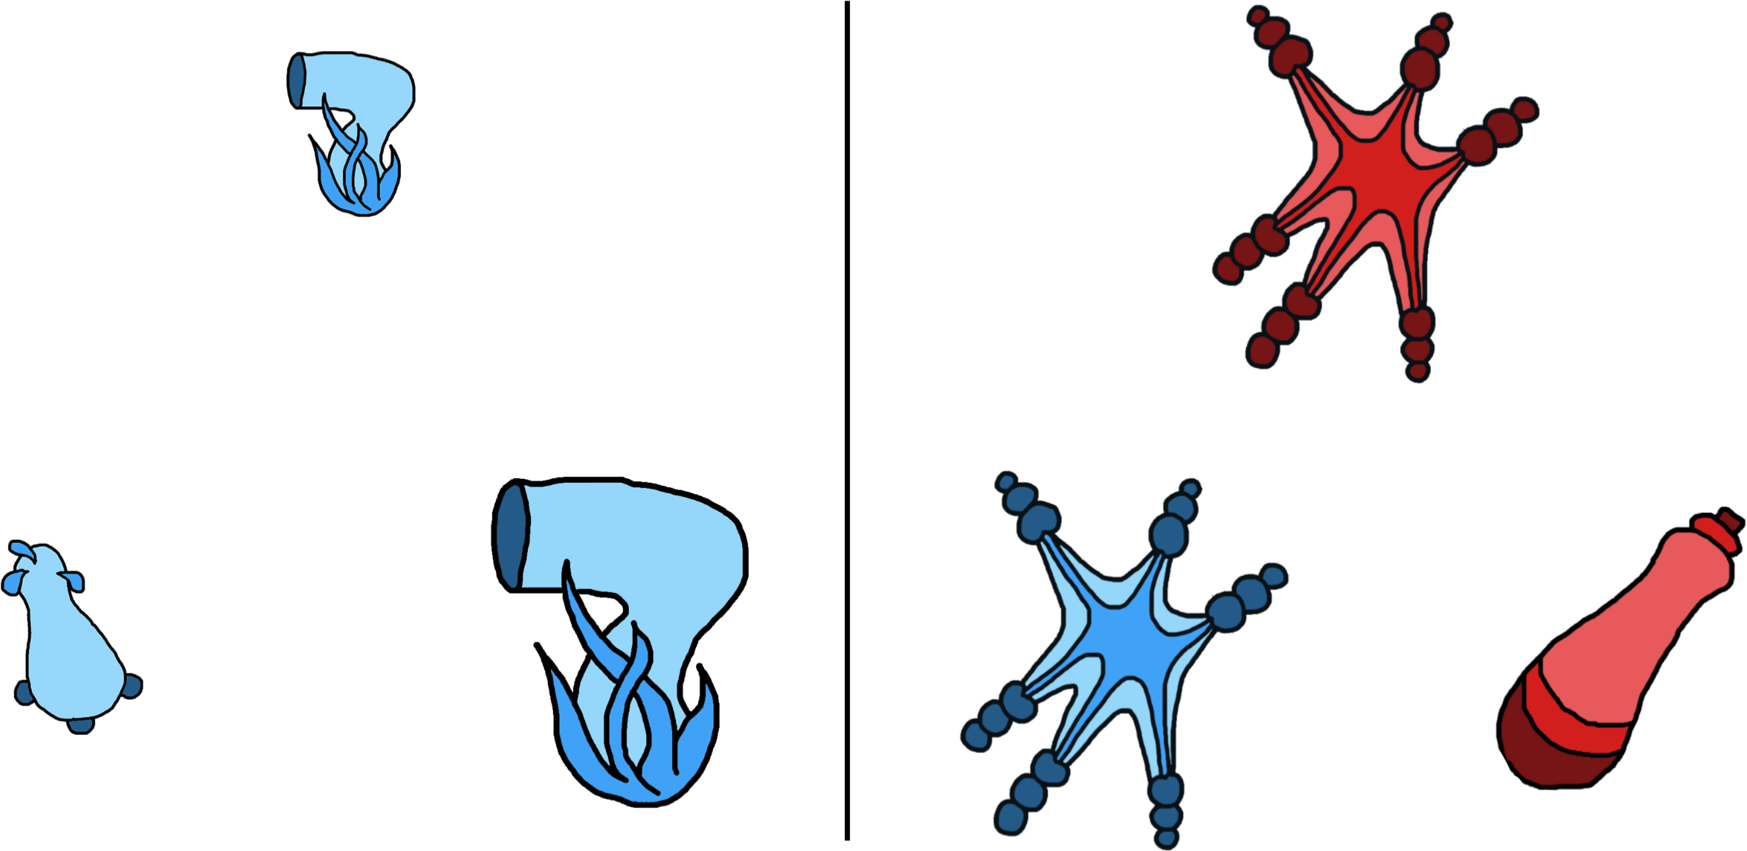
\includegraphics{figs/colortrial-1} 

}

\caption{On the left: an example of a contrastive display in which the feature type is color. Here, the participant would hear the instruction, e.g., ``Find the toma'' or ``Find the red toma.'' The target is the red star-shaped object.  On the right:  an example of a contrastive display in which the feature type is size. Here, the participant would hear the instruction, e.g., ``Find the toma'' or ``Find the small toma.'' The target is the small hairdryer-shaped object. In each case, the lure shares the target's feature (red on the left, small on the right) but not its shape. The contrastive pair shares the target's shape but not its feature. Labels of the target and lure are provided for clarity and were not shown to participants.}\label{fig:colortrial}
\end{figure}

\hypertarget{method}{%
\subsection{Method}\label{method}}

\hypertarget{participants.}{%
\subsubsection{Participants.}\label{participants.}}

We recruited a pre-registered sample of 300 participants through Amazon Mechanical Turk. Each participant gave informed consent and was paid \$0.30 in exchange for their participation. Participants were told the task was estimated to take 3 minutes and on average they took 44 seconds to complete the task (not including reading the consent form).

\hypertarget{stimuli.}{%
\subsubsection{Stimuli.}\label{stimuli.}}

Stimulus displays were arrays of three novel fruit objects. We chose alien fruits as stimuli because fruits are a superordinate category that can intuitively vary considerably in shape, color, and size. Fruits were selected randomly at each trial from 20 fruit kinds. Ten of the 20 fruit drawings were adapted and redrawn from Kanwisher, Woods, Iacoboni, and Mazziotta (1997); we designed the remaining 10 fruit kinds. Each fruit kind had an instance in each of four colors (red, blue, green, or purple) and two sizes (big or small). Particular target colors were assigned randomly at each trial and particular target sizes were counterbalanced across contrastive displays vs.~filler trials. The on-screen positions of the target and distractor items were randomized within a triad configuration.

Our trials of interest were contrastive displays: displays with a contrastive pair, which allows for a contrastive inference. Contrastive displays contained a target, its contrastive pair (which matched the target's shape but not its feature), and a lure (which matched the target's feature but not its shape; Fig. \ref{fig:colortrial}).

We also included unique target displays as filler trials. Unique target displays contained a target object that had a unique shape and a unique feature value (color or size), and two distractor objects that matched each other's (but not the target's) shape and feature. Unique target displays were included to space out contrastive displays and to prevent participants from dialing in on the intended contrastive inference during the experiment. Further details about these trials, and the analysis of participants' choices in them, can be found in the Supplemental Materials. All discussion of the results in the main text include only the contrastive displays.

In summary, we manipulated utterance type (\emph{noun} or \emph{adjective noun}) and feature type (color or size). Utterance type was manipulated within subjects, as utterance type is the central manipulation of interest. Feature type (color or size) was manipulated between subjects, to keep the number of unique novel stimuli to be generated manageable given the constraint that each participant could not be shown any stimulus shape on more than one trial.

\hypertarget{design-and-procedure.}{%
\subsubsection{Design and Procedure.}\label{design-and-procedure.}}

Participants were told they would play a game in which they would search for strange alien fruits. There were eight trials in total. Half of the trials were contrastive displays and half were unique target displays (filler trials). Half of trials had audio instructions with no adjective (e.g., ``Find the toma''; the \emph{noun} utterance type), and half of trials had audio instructions with an adjective that described the critical feature of the target (e.g., ``Find the red toma'' or ``Find the small toma''; the \emph{adjective noun} utterance type). A label was randomly chosen at each trial from a list of eight novel words: blicket, wug, toma, gade, sprock, koba, zorp, and lomet.

After completing the study, as a check of their attention to the task, participants were asked to select which of a set of alien words they had heard previously during the study. Four were words they had heard, and four were novel lure words. Participants were dropped from further analysis if they did not meet our pre-registered exclusion criteria of responding to at least 6 of these 8 check items correctly (above chance performance as indicated by a one-tailed binomial test at the \(p = .05\) level) and answering four simple color perception check trials correctly (resulting \(n =\) 163)\footnote{Experiments 1 and 3 were run in 2020, during the COVID-19 pandemic, when high exclusion rates on Amazon Mechanical Turk were being reported by many experimenters. Though our pre-registered criteria led to many exclusions, the check given to participants tested memory for a few novel words heard in the experiment, which we do not believe was an overly stringent requirement.}.

\hypertarget{results}{%
\subsection{Results}\label{results}}

\begin{figure}[!tb]

{\centering \includegraphics{figs/e1-webppl-plot-1} 

}

\caption{Proportion of times that people (and our model) chose the target and lure items, depending on utterance type (noun vs. adjective noun) and feature type (color vs. size). The top row depicts example trials (repeated from Fig. 1). Points indicate empirical means; error bars indicate 95\% confidence intervals computed by non-parametric bootstrapping. Solid horizontal lines indicate model predictions.}\label{fig:e1-webppl-plot}
\end{figure}

Our key pre-registered analysis was whether participants would choose the target object when they heard an adjective in the referring expression. For example, when they saw the stimuli in the right panel of Figure \ref{fig:colortrial} and heard ``Find the small toma,'' would they choose the target (small hairdryer-shaped object) over the lure (small pear-shaped object)? To perform this test, we compared participants' rate of choosing the target to their rate of choosing the lure, which shares the relevant feature with the target, on \emph{adjective noun} trials. Overall, participants chose the target more often than the lure, indicating that they used contrastive inferences to resolve reference (\(\beta =\) 0.53, \(t =\) 3.83, \(p =\) \textless{} .001). That is, overall, they tended to choose the red star-shaped object over the red zucchini-shaped object in the left panel of Figure \ref{fig:colortrial}, and tended to choose the small hairdryer-shaped object over the small pear-shaped object in the right panel. To test whether the strength of the contrastive inference differed between color and size, we pre-registered a version of this regression with a term for feature type, and found that people were more likely to choose the target over the lure in the size condition than the color condition (\(\beta =\) 0.87, \(t =\) 3.12, \(p =\) .002). That is, referring again to the displays in Figure \ref{fig:colortrial}, people were less likely to choose the target when hearing ``Find the red toma'' and choosing among items on the left, and more likely to choose the target object when hearing ``Find the small toma'' and picking among the items on the right. Overall, when people hear an utterance like ``red toma'' or ``small toma'', they tend to choose the target over the lure, and this tendency is stronger with size adjectives than color adjectives (Fig. \ref{fig:e1-webppl-plot}).

Given this result, we tested whether people consistently chose the target over the lure in \emph{adjective noun} trials in the color and size conditions separately, as a stricter check of whether the effect was present in both feature types (not pre-registered). Considering color and size separately, participants did not choose the target significantly more often than the lure in the color condition (\(\beta =\) 0.15, \(t =\) 0.75, \(p =\) .455), but did choose the target significantly more often than the lure in the size condition (\(\beta =\) 0.86, \(t =\) 4.41, \(p =\) \textless{} .001).

When there was no adjective in the utterance (\emph{noun} trials), participants dispreferred the target, instead choosing the lure object, which matched the target's feature but had a unique shape (\(\beta =\) -2.65, \(t =\) -5.44, \(p =\) \textless{} .001). That is, when people hear an utterance like ``Find the toma,'' they tend to choose the lure (Fig. \ref{fig:e1-webppl-plot}): the zucchini-shaped object in the left panel and the pear-shaped object in the right panel of Figure \ref{fig:colortrial}. Participants' choice of the target in \emph{adjective noun} trials in the size condition was therefore not due to a prior preference for the target, but relied on contrastive interpretation of the adjective. In the Supplemental Materials, we report an additional pre-registered analysis of all Experiment 1 data with maximal terms and random effects; those results are consistent with the more focused tests reported here.

\hypertarget{discussion}{%
\subsection{Discussion}\label{discussion}}

When faced with unfamiliar objects referred to by unfamiliar words, people can use pragmatic inference to resolve referential ambiguity and learn the meanings of new words. In Experiment 1, we found that people have a general tendency to choose objects that are unique in shape when reference is ambiguous: when they see a display like those in Figure \ref{fig:colortrial} and hear ``Find the toma,'' they tend to choose the lure. However, when they hear an utterance with an adjective (e.g., ``Find the red toma'', ``Find the small toma''), they shift away from choosing the unique lure and toward choosing the target, which has a similar contrasting counterpart. Furthermore, use of size adjectives---but not color adjectives---prompts people to choose the target object significantly more often than the lure object. We found that people are able to use contrastive inferences about size to successfully resolve which unfamiliar object an unfamiliar word refers to.

\hypertarget{model}{%
\subsection{Model}\label{model}}

To formalize the inference that participants were asked to make, we developed a model in the Rational Speech Act Framework (RSA, Frank \& Goodman, 2012).\footnote{We implemented these models in the WebPPL programming language (Goodman \& Stuhlmüller, 2014), using analyses informed by Scontras, Tessler, and Franke (2018) and using the Rwebppl package (Braginsky, Tessler, \& Hawkins, 2019).} In this framework, pragmatic listeners (\(L\)) are modeled as drawing inferences about speakers' (\(S\)) communicative intentions in talking to a hypothetical literal listener (\(L_{0}\)). This literal listener makes no pragmatic inferences at all: it evaluates the literal truth of a statement (e.g., it is true that a red toma can be called ``toma'' and ``red toma'' but not ``blue toma'') and chooses randomly among all referents consistent with that statement. In planning their referring expressions, speakers choose utterances that are successful at accomplishing two goals: (1) making the listener as likely as possible to select the correct object, and (2) minimizing their communicative cost (i.e., producing as few words as possible). Note that though determiners are not given in the model's utterances, the assumption that the utterance refers to a specific referent is built into the model structure, consistent with the definite determiners used in the task. Pragmatic listeners use Bayes' rule to invert the speaker's utility function, essentially inferring what the speaker's intention was likely to be given the utterance they produced.

\[Literal: P_{Lit} = \delta\left(u,r\right)P\left(r\right)\]
\[Speaker: P_S\left(u \vert r\right) \propto \alpha \left(P_{Lit}\left(r \vert u\right) - C\right)\]
\[Listener: P_{Learn}\left(r \vert u\right) \propto P_s\left(u \vert r\right)P\left(r\right)\]

For this experiment, we build on a Rational Speech Act model developed by Frank and Goodman (2014) to jointly resolve reference and learn new words. The primary modification of RSA is the use of a pragmatic \emph{learner}: a pragmatic listener who has uncertainty about the meanings of words in their language, and thus cannot directly compute the speaker's utility as written. Instead, the speaker's utility is conditioned on the set of mappings between words and meanings, and the learner must also infer which set of mappings is correct:\\
\[Learner: P_L\left(r \vert u\right) \propto P_s\left(u \vert r; m\right)P\left(r\right)P\left(m\right)\]

In these experiments, we assume that the prior probability to refer to each object \((P\left(r\right))\) is equal, and similarly that all mappings \((P\left(m\right))\) are equally likely, so they cancel out in computations. We further assume that the cost of producing any word is identical, and so the cost of an utterance is equal to its length. All that remains is to specify the possible mappings, and literal meanings, and alternative utterances possible on each trial of the experiment. We describe the size condition here, but the computation for the color condition is analogous.

On the trial shown in the right panel of Figure \ref{fig:colortrial}, people see two objects that look something like a hairdryer and one that looks like a pear, and they are asked to ``Find the toma.'' Here, in the experiment design and the model, we take advantage of the fact that English speakers tend to assume that nouns generally correspond to differences in shape rather than other features (Landau, Smith, \& Jones, 1992). Given this, the two possible mappings are \(\{m_1: hairdryer-``toma", pear-?\}\) and \(\{m_2: hairdryer-?, pear-``toma"\}\). The literal semantics of each object allow them to be referred to by their shape label (e.g.~``toma''), or by a adjective that is true of them (e.g.~``small''), but not names for other shapes or untrue adjectives.

Having heard ``Find the toma,'' the model must now choose a referent. If the true mapping for ``toma'' is the hairdryer shape (\(m_1\)), this utterance is ambiguous to the literal listener, as there are two referents consistent with the literal meaning toma. Consequently, whichever of the two referents the speaker intends to point out to the learner, the speaker's utility will be relatively low. Alternatively, if the true mapping for ``toma'' is the pear shape (\(m_2\)), then the utterance will be unambiguous to the literal listener, and thus the speaker's utterance will have higher utility. As a result, the model can infer that the more likely mapping is \(m_2\) and choose the pear-shaped object, simultaneously resolving reference and learning the meaning of ``toma.''

If instead the speaker produced ``Find the small toma,'' the model will make a different inference. If the true mapping for ``toma'' is the hairdryer shape (\(m_2\)), this utterance now uniquely identifies one referent for the literal listener and thus has high utility. It also uniquely identifies the target if ``toma'' means pear shape (\(m_1\)). However, if ``toma'' means pear shape, the speaker's utterance was inefficient because the single word utterance ``toma'' would have identified the target to the literal listener and incurred less cost. Thus, the model can infer that ``toma'' is more likely to mean hairdryer shape and choose the small hairdryer-shaped object appropriately.

While these descriptions use deterministic language for clarity, the model's computation is probabilistic and thus reflects tendencies to choose those objects rather than fixed rules. Figure \ref{fig:e1-webppl-plot} shows model predictions alongside people's behavior in Experiment 1. In line with the intuition above, the model predicts that hearing just a noun (e.g.~``toma''; \emph{noun} utterance type) should lead people to infer that the intended referent is the unique object (lure), whereas hearing a modified noun (e.g.~``small toma''; \emph{adjective noun} utterance type) should lead people to infer that the speaker's intended referent has a same-shaped counterpart without the described feature (i.e., is the target object).

Our empirical data suggest that people treat color and size adjectives differently, making a stronger contrastive inferences about size than color. In the Rational Speech Act model, this kind of difference can be captured by the rationality parameter \(\alpha\), which adjusts how sensitive the speaker is to differences in utility of different utterances. We estimated the rationality parameter separately for color and size to account for this difference and better fit the data. Note that we are using this parameter to approximate people's behavior and do not ascribe a particular psychological interpretation to it; we describe below some alternative modeling choices that could derive color--size asymmetries with more principled interpretations about people's reasoning processes.

To determine the value of the feature rationality parameter that best describes participants' behavior in each condition, we used Bayesian data analysis, estimating the posterior probability of the observed data under each possible value of \(\alpha\) multiplied by the prior probability of each of those values. To estimate the parameter value in each condition, \(\alpha\) was drawn from a Gamma distribution with shape and scale parameters set to 2 (\(Gamma\left(2,2\right)\)), and we sampled using Markov Chain Monte Carlo (MCMC) sampling. This prior encodes a weak preference for small values of \(\alpha\), but the estimates below were not sensitive to other choices of hyper-parameters. Posterior mean estimates of the feature rationality parameter varied substantially across conditions. In the color condition, the feature rationality parameter was estimated to be 2.00 with a 95\% credible interval of {[}1.37, 2.63{]}. In the size condition, the feature rationality parameter was estimated to be 3.98 {[}3.22, 4.74{]}.

Figure \ref{fig:e1-webppl-plot} shows the model predictions along with the empirical data from Experiment 1. The model broadly captures the contrastive inference: when speakers produce an \emph{adjective noun} utterance like ``red toma,'' the model selects the target object more often than the lure object. The different estimated feature rationality values also allow the model to capture that people make stronger contrastive inferences about size than color. However, in both conditions, the model overpredicts the extent of the contrastive inference that people make. Intuitively, it appears that over and above the strength of their contrastive inferences, people have an especially strong tendency to choose a unique object when they hear an unmodified noun (i.e., to choose the lure in the \emph{noun} condition). In an attempt to capture this uniqueness tendency, the model overpredicts the extent of the contrastive inference (choice of the target in the \emph{adjective noun} condition).

Why do people make stronger pragmatic inferences about size than color when determining reference? Our model implements this difference in a relatively agnostic way, and these data alone cannot arbitrate between particular explanations, but we spell out a few possibilities and modeling alternatives here.

One way to capture this asymmetry would be to locate it in a different part of the model: in the literal semantics of color and size. A recent model from Degen, Hawkins, Graf, Kreiss, and Goodman (2020) does predict a color--size asymmetry based on different semantic exactness. In this model, literal semantics are treated as continuous rather than discrete, so ``blue'' is neither 100\% true nor 100\% false of a particular object, but can instead be 90\% true. They successfully model a number of color--size asymmetries in production data by treating color as having stronger literal semantics (e.g.~``blue toma'' is a better description of a small blue toma than ``small toma'' is). A continuous semantics model with stronger literal semantics for color than size can capture the key asymmetry between color and size in the \emph{adjective noun} trials---that people make more consistent contrastive inferences about size than color---because speakers are expected to mention color more often. However, when fitting a continuous semantics model to all of our data (\emph{noun} and \emph{adjective noun} trials), we do not find the expected strength of semantic values (as demonstrated in the Supplemental Materials). This may be because of people's choice patterns in the \emph{noun} trials as well as their generally noisy guessing. Overall, this approach is a promising avenue for accounting for color--size asymmetries, but may need additional adjustments to account for people's choice patterns in a highly ambiguous task like this one.

Another possibility is that people's different inferences about size and color adjectives are explained by the gradable semantics of size. Size adjectives are relative gradable adjectives: their meaning is judged relative to a comparison class (e.g., ``He is a tall basketball player'' may have a meaning akin to ``He is tall for a basketball player'') (Kennedy, 2007). Because this comparison class is sensitive to context (it can even change within a sentence, e.g., ``He is tall, but not tall for a basketball player''), there is active disagreement about whether this aspect of gradable adjective meaning is properly considered semantics or pragmatics, or encompasses both semantic and pragmatic processes (Tessler, Tsvilodub, Snedeker, \& Levy, 2020; Xiang, Kennedy, Xu, \& Leffel, 2022). A gradable semantics account of our finding would posit that a comparison class is necessary to judge size but not color, which accounts for the asymmetry. This would accord with work in which the presence of a local comparison class facilitates reference resolution among familiar objects described with relative adjectives (Aparicio et al., 2016). That is, in a trial such as the one on the right in Figure \ref{fig:colortrial}, a participant sees two hairdryer-shaped objects, one big and one small, and one small pear-shaped object. When they hear ``Find the small toma,'' they choose the only object that is small and has a potential known comparison class: the small hairdryer-shaped object, which has a larger hairdryer-shaped counterpart. On the other hand, color adjectives are not relative gradable adjectives, and so a comparison class is not necessary to interpret them: they have more absolute meaning. Thus, it is possible to explain the color--size asymmetry by the necessity of a comparison class for judging size, and this may be attributed to semantics, pragmatics, or a combination of both.

Overall, we found that people can use contrastive inferences from description to map an unknown word to an unknown object. This inference is captured by an extension of the Rational Speech Act model using a pragmatic learner, who is simultaneously making inferences over possible referents and possible lexicons. This model can also capture people's tendency to make stronger contrastive inferences from color description than size description through differences in the rationality parameter, though the origin of these differences cannot be pinned down with this experiment alone. Our experiment and model results suggest that people can resolve a request like ``Give me the small toma'' by reasoning that the speaker must have been making a useful distinction by mentioning size, and therefore looking for multiple similar objects that differ in size and choosing the smaller one. Immediately available objects are not the only ones worth making a distinction from, however. Next, we turn to another salient set of objects a speaker might want to set a referent apart from: the referent's category.

\hypertarget{experiment-2}{%
\section{Experiment 2}\label{experiment-2}}

When referring to a \emph{big red dog} or a \emph{hot-air balloon}, we often take care to describe them---even when there are no other dogs or balloons around. Speakers use more description when referring to objects with atypical features (e.g., a yellow tomato) than typical ones (e.g., a red tomato; Mitchell et al., 2013; Bergey, Morris, \& Yurovsky, 2020; Rubio-Fernández, 2016; Westerbeek et al., 2015). This selective marking of atypical objects potentially supplies useful information to listeners: they have the opportunity to not only learn about the object at hand, but also about its broader category.

Horowitz and Frank (2016) demonstrated that, combined with other contrastive cues (e.g., ``Wow, this one is a zib. This one is a TALL zib''), prenominal adjectives prompted adults and children to infer that the described referent was less typical than one that differed on the mentioned feature (e.g., a shorter zib). This work provided a useful demonstration that adjective use can contribute to inferences about feature typicality, though it did not isolate the effect of adjectives specifically. Their experiments used several contrastive cues, such as prosody (contrastive stress on the adjective: ``TALL zib''), demonstrative phrases that may have marked the object as unique (``this one'') and expressions of surprise at the object (``wow''), and participants may have inferred the object was atypical primarily from these cues and not from the adjective. Thus, in this experiment, we first set out to ask whether adjective use alone prompts an inference of atypicality: when you hear ``purple toma,'' do you infer that \emph{fewer} tomas in general are purple?

We will also test how this inference differs (or does not) between size and color adjectives. The fact that people use adjectives to draw a contrast between an object and its category may help make sense of the asymmetry between color and size adjectives we found in Experiment 1. Color adjectives that are redundant with respect to reference are not necessarily redundant in general. Rubio-Fernández (2016) demonstrates that speakers often use `redundant' color adjectives to describe colors when they are variable and central to the category's meaning (e.g., colorful t-shirts) or when they are atypical (e.g., a purple banana). Comprehenders, in turn, expect color adjectives to be used informatively with respect to typicality, and upon hearing color adjectives tend to look to referents for which the adjective describes a less-typical feature (e.g., ``Choose the yellow\ldots'' prompts people to orient to a yellow shirt over a yellow banana; Rohde \& Rubio-Fernandez, 2021; Kreiss \& Degen, 2020). Therefore, while size may hold more contrastive weight than color with respect to reference (as shown in Experiment 1), color and size may hold similar contrastive weight with respect to conveying atypicality. If so, size and color adjectives should prompt inferences of atypicality to a similar degree. In Experiment 2, we test whether listeners use descriptive contrast with a novel object's category to learn about the category's feature distribution.

If listeners do make contrastive inferences about typicality, it may not be as simple as judging that an over-described referent is atypical. Description can serve many purposes: in Experiment 1, we investigated its use in contrasting between present objects. If an adjective was needed to distinguish between two present objects, it may not have been used to mark atypicality. For instance, in the context of a bin of heirloom tomatoes, a speaker who wanted a red one in particular might specify that they want a ``red tomato'' rather than just asking for a ``tomato.'' In this case, the adjective ``red'' is being used contrastively with respect to reference (as in Experiment 1), and not to mark atypicality. Thus, a listener who does not know much about tomatoes may attribute the use of ``red'' to referential disambiguation given the context and not infer that red is an unusual color for tomatoes.

In Experiment 2, we used a task with novel objects to set up just this kind of learning situation. We manipulated the contexts in which listeners hear adjectives modifying novel names of novel referents. These contexts varied in how useful the adjective was to identify the referent: in one context the adjective was necessary, in another it was helpful, and in a third it was entirely redundant. On a \emph{reference-first view}, use of an adjective that was necessary for reference can be explained away and should not prompt further inferences about typicality---an atypicality inference would be blocked. If, on the other hand, people take into account speakers' multiple reasons for using adjectives without giving priority to reference (the \emph{probabilistic weighing view}), they may alter their inferences about typicality across these contexts in a graded way: if an adjective was necessary for reference, it may prompt slightly weaker inferences of atypicality; if an adjective was redundant with respect to reference, it may be inferred to mark atypicality more strongly. Further, these contexts may also prompt distinct inferences when no adjective is used: for instance, when an adjective is necessary to identify the referent but elided, people may infer that the elided feature is particularly typical. To account for the multiple ways context effects might emerge, we analyze both of these possibilities. Overall, we asked whether listeners infer that adjectives mark atypical features of objects, and whether the strength of this inference depends on the referential ambiguity of the context in which the adjectives are used.

\begin{figure}
\centering
\includegraphics{figs/e2-aliens-1.pdf}
\caption{\label{fig:e2-aliens}Experiment 2 stimuli. In the above example, the critical feature is size and the object context is a within-category contrast: the alien on the right has two same-shaped objects that differ in size.}
\end{figure}

\hypertarget{method-1}{%
\subsection{Method}\label{method-1}}

\hypertarget{participants.-1}{%
\subsubsection{Participants.}\label{participants.-1}}

240 participants were recruited from Amazon Mechanical Turk. Half of the participants were assigned to a condition in which the critical feature was color (red, blue, purple, or green), and the other half of participants were assigned to a condition in which the critical feature was size (small or big). Participants were paid \$0.30. Participants were told the task was estimated to take 3 minutes and on average took 118 seconds to complete the task (not including reading the consent form).

\hypertarget{stimuli-procedure.}{%
\subsubsection{Stimuli \& Procedure.}\label{stimuli-procedure.}}

Stimulus displays showed two alien interlocutors, one on the left side (Alien A) and one on the right side (Alien B) of the screen, each with two novel fruit objects beneath them (Figure \ref{fig:e2-aliens}). Alien A, in a speech bubble, asked Alien B for one of its fruits (e.g., ``Hey, pass me the big toma''). Alien B replied, ``Here you go!'' and the referent disappeared from Alien B's side and reappeared on Alien A's side. Note that the participants do not make a referent choice in this experiment; the measure of interest is their typicality judgments of the objects' features, described below.

We manipulated three factors: utterance type, feature type, and context type. As in Experiment 1, we prioritized utterance type as a within-subjects manipulation because it was the central manipulation of interest. We also prioritized context type because another central question was whether context would alter the effect of utterance. We manipulated the critical feature type (color or size) between subjects, as in Experiment 1, to maximize our use of the set of novel stimuli without showing any participant the same novel shape on more than one trial.

Utterance type and context type were fully crossed within subjects. Utterance type had two levels: \emph{noun} (e.g., ``Hey, pass me the toma'') or \emph{adjective noun} (e.g., ``Hey, pass me the big toma'' or ``Hey, pass me the blue toma''). Context type had three levels: within-category contrast, between-category contrast, and same feature (Figure \ref{fig:e2-wppl-plot}). In the within-category contrast condition, Alien B possessed the target object and another object of the same shape, but with a different feature value (e.g., a big toma and a small toma). In the between-category contrast condition, Alien B possessed the target object and another object of a different shape, and with a different feature value (e.g., a big toma and a small blicket). In the same feature condition, Alien B possessed the target object and another object of a different shape and with the same feature as the target (e.g., a big toma and a big dax). Thus, in the within-category contrast condition, the descriptor was necessary to distinguish the referent; in the between-category contrast condition it was unnecessary but potentially helpful; and in the same feature condition it was unnecessary and unhelpful.

Note that in all context conditions, the set of objects on screen was the same in terms of the experiment design: there was a target (e.g., big toma), an object with the same shape as the target and a different critical feature (e.g., small toma), an object with a different shape from the target and the same critical feature (e.g., big dax), and an object with a different shape from the target and a different critical feature (e.g., small blicket). Context was manipulated by rearranging these objects such that the relevant referents (the objects under Alien B) differed and the remaining objects were under Alien A. Thus, in each case, participants saw the target object and one other object that shared the target object's shape but not its critical feature--they observed the same kind of feature distribution of the target object's category in each trial type. The particular values of the features were chosen randomly for each trial, and the particular object shapes were chosen randomly among a set of 24 novel fruit shapes.

Participants completed six trials. After each exchange between the alien interlocutors, they made a judgment about the prevalence of the target's critical feature in the target object's category. This prevalence judgment, on a 0-100\% scale, is our measure of interest. For instance, after seeing a blue toma being exchanged, participants would be asked, ``On this planet, what percentage of tomas do you think are blue?'' They would answer on a sliding scale between zero and 100. In the size condition, participants were asked, ``On this planet, what percentage of tomas do you think are the size shown below?'' with an image of the target object they just saw available on the screen.

After completing the study, participants were asked to select which of a set of alien words they had seen previously during the study, as a check of whether they attended to the task. Four were words they had seen, and four were novel lure words. Participants were dropped from further analysis if they did not respond to at least 6 of these 8 correctly (above chance performance as indicated by a one-tailed binomial test at the \(p = .05\) level). This resulted in excluding 47 participants, leaving 193 for further analysis.

\hypertarget{results-1}{%
\subsection{Results}\label{results-1}}

Our key test is whether participants infer that a mentioned feature is less typical than one that is not mentioned. In addition, we tested whether inferences of atypicality are modulated by context. One way to test this is to analyze the interaction between utterance type and context, seeing if the difference between adjective and no adjective utterances is larger when the adjective was highly redundant or smaller when the adjective was necessary for reference.

We analyzed participants' judgments of the prevalence of the target object's critical feature in its category. We began by fitting a maximum mixed-effects linear model with effects of utterance type (\emph{noun} or \emph{adjective noun}), context type (within category, between category, or same feature, with between category as the reference level), and critical feature (color or size) as well as all interactions and random slopes of utterance type and context type nested within subject. Random effects were removed until the model converged. The final model included the effects of utterance type, context type, and critical feature and their interactions, and a random slope of utterance type by subject. This model revealed a significant effect of utterance type (\(\beta_{adjective} =\) -10.22, \(t =\) -3.37, \(p =\) .001), such that prevalence judgments were lower in the \emph{adjective noun} trials than the \emph{noun} trials. That is, when people saw the alien say ``Pass me the big toma'' or ``Pass me the blue toma,'' they judged that tomas were less likely to be big or blue, respectively, than when those features were not mentioned. Participants' inferences did not significantly differ between color and size adjective conditions (\(\beta_{size} =\) 4.73, \(t =\) 1.46, \(p =\) .146). Participants' inferences did not significantly vary by context type (\(\beta_{within} =\) 3.92, \(t =\) 1.63, \(p =\) .104; \(\beta_{same} =\) -1.48, \(t =\) -0.62, \(p =\) .537), though numerically they made higher prevalence judgments in the within-category context. There was not a significant interaction between context and presence of an adjective in the utterance (\(\beta_{within*adjective} =\) -1.58, \(t =\) -0.46, \(p =\) .644; \(\beta_{same*adjective} =\) 2.13, \(t =\) 0.63, \(p =\) .532). That is, participants did not significantly adjust their inferences based on object context, nor did they make differential inferences based on the combination of context and adjective use. However, they robustly inferred that mentioned features were less prevalent in the target's category than unmentioned features.

This lack of a context effect may be because people do not take context into account, or because they make distinct inferences when an adjective is \emph{not} used: for instance, when an adjective is necessary for reference but elided, people may infer that the unmentioned feature is very typical. This inference would lead to a difference between the \emph{noun} and \emph{adjective noun} utterances in the within-category context, but not because people are failing to attribute the adjective to reference. To account for this possibility, we separately tested whether there are effects of context among just the \emph{noun} trials and just the \emph{adjective noun} trials. In each case, we fit a model with effects of context type and critical feature as well as their interaction and random slopes by subject.
Participants did not significantly adjust their inferences by context among only the \emph{noun} trials (\(\beta_{within} =\) 3.94, \(t =\) 1.47, \(p =\) .143; \(\beta_{same} =\) -1.46, \(t =\) -0.54, \(p =\) .587), though numerically they made higher prevalence judgments in the within-category context. That is, we did not find evidence here that people were inferring a feature to be highly typical because it went unmentioned when it was necessary for reference. Participants also did not significantly adjust their inferences by context among only the \emph{adjective noun} trials (\(\beta_{within} =\) 2.43, \(t =\) 1.16, \(p =\) .247; \(\beta_{same} =\) 0.67, \(t =\) 0.32, \(p =\) .750), though their judgments were numerically higher in the within-category context. That is, we did not find evidence that people modulated their typicality inferences based on the referential context among trials where this inference could not have been driven by omission either. Overall, we did not find evidence that participants significantly adjusted their inferences based on context.

\hypertarget{discussion-1}{%
\subsection{Discussion}\label{discussion-1}}

Description is often used not to distinguish among present objects, but to pick out an object's feature as atypical of its category. In Experiment 2, we asked whether people would infer that a described feature is atypical of a novel category simply because it was mentioned. We found that people robustly inferred that a mentioned feature was atypical of its category, across both size and color description. Further, participants did not use object context to substantially explain away description. That is, even when description was necessary to distinguish among present objects (e.g., there were two same-shaped objects that differed only in the mentioned feature), participants still inferred that the feature was atypical of its category. This suggests that, in the case of hearing someone ask for a ``red tomato'' from a bin of many-colored heirloom tomatoes, a person naive about tomatoes would infer that tomatoes are relatively unlikely to be red.

Unlike in Experiment 1, in which people made stronger contrastive inferences about size than color, there were not substantial differences between people's inferences about color and size in Experiment 2. If an account based on production norms is correct, this suggests that people track both how often people use color compared to size description and also for what purpose---contrasting with present objects or with the referent's category. That is, color description may be more likely to be used superfluously with respect to present objects but informatively with respect to the category. Indeed, color description that seems overdescriptive with respect to object context often occurs when the category has many-colored members (e.g., t-shirts) or when the object's color is atypical (Rubio-Fernández, 2016). However, our results are consistent with several potential explanations of the color-size asymmetry (or lack thereof). Future work addressing the source of the color-size asymmetry will need to explain differences in its extent when distinguishing among present objects compared to the referent's category.

Another interpretation of people's inferences in the size condition is that they are due to size adjectives being relative gradable adjectives. That is, the phrases ``big toma'' and ``small toma'' may inherently carry the meaning ``big for a toma'' and ``small for a toma'' (which can be interpreted as an aspect of the adjective's semantics, not pragmatics; see discussion in Experiment 1). It is possible to attribute people's atypicality inferences in the size condition to the relative gradable nature of size adjectives. However, people also made these inferences about color adjectives, which are not relative gradable adjectives. A purely semantic account also might predict that people's inferences about color and size would be different---for instance, that people would make larger atypicality inferences about size than color---which we do not find. Though the semantics of size adjectives may contribute to people's inferences of atypicality in the size condition, we find it parsimonious here to explain the color and size inferences by the same mechanism---pragmatic reasoning.

\hypertarget{model-1}{%
\subsection{Model}\label{model-1}}

To allow the Rational Speech Act Framework to capture inferences about typicality, we modified the Speaker's utility function to have an additional term: the listener's expected processing difficulty. Speakers may be motivated to help listeners to select the correct referent not just eventually but as quickly as possible. Speakers are sensitive to factors that affect listeners' processing difficulty (Long, Moore, Mollica, \& Rubio-Fernandez, 2021), and speaker behavior can be captured by modeling listeners' visual search for a referent (Jara-Ettinger \& Rubio-Fernandez, 2022). People are both slower and less accurate at identifying atypical members of a category as members of that category (Dale, Kehoe, \& Spivey, 2007; Rosch, Simpson, \& Miller, 1976). If speakers account for listeners' processing difficulties, they should be unlikely to produce bare nouns to refer to low typicality exemplars (e.g., unlikely to call a purple carrot ``carrot'').

We model the speaker as reasoning about the listener's label verification process. Because the speed of verification scales with the typicality of a referent, a natural way of modeling it is as a process of searching for that particular referent in the set of all exemplars of the named category, or alternatively of sampling that particular referent from the set of all exemplars in that category, \(P\left(r \vert Cat\right)\). On this account, speakers want to provide a modifying adjective for atypical referents because the probability of sampling them from their category is low, but the probability of sampling them from the modified category is much higher (a generalization of the size principle, Xu and Tenenbaum (2007)). Typicality is just one term in the speaker's utility, and thus is directly weighed with the literal listener's judgment and against cost. Note that modeling typicality as part of the speaker's reasoning about listener processing will make similar predictions to integrating typicality into the semantics of the literal listener (as in Degen et al., 2020).

If speakers use this utility function, a listener who does not know the feature distribution for a category can use a speaker's utterance to infer it. Intuitively, a speaker should prefer not to modify nouns with adjectives because they incur a cost for producing an extra word. If they did use an adjective, it must be because they thought the learner would have a difficult time finding the referent from a bare noun alone because of typicality, competing referents, or both. To infer the true prevalence of the target feature in the category, learners combine the speaker's utterance with their prior beliefs about the feature distribution.

We model the learner's prior about the prevalence of features in any category as a \(\text{Beta}\) distribution with two parameters \(\alpha\) and \(\beta\) that encode the number of hypothesized prior psuedo-exemplars with the feature and without feature that the learner has previously observed (e.g., one blue toma and one red toma or one big toma and one small toma). (Note that the \(\alpha\) parameter of this \(\text{Beta}\) distribution is distinct from the \(\alpha\) used to represent the rationality parameter.) We assume that the learner believes they have previously observed one hypothetical psuedo-examplar of each type, which is a weak symmetric prior indicating that the learner expects features to occur in half of all members of a category on average, but would find many levels of prevalence unsurprising. To model the learner's direct experience with the category, we add the observed instances in the experiment to these hypothesized prior instances. After observing one member of the target category with the relevant feature and one without, the listener's prior is thus updated to be \(\text{Beta}\left(2,\,2\right)\). Thus, we model learners as believing the feature prevalence is roughly 50\% based on their initial priors and direct observation in the trial; they then combine this knowledge of the feature distribution with their pragmatic inference about the utterance to arrive at a final prevalence judgment.

As in Experiment 1, we encoded potential differences between people's inferences about color and size in feature rationality parameters, which we estimated separately for Experiment 2. To determine the value of the feature rationality parameter that best describes participants' behavior in each condition, we again used Bayesian data analysis, estimating the posterior probability of the observed data under each possible value of \(\alpha\) multiplied by the prior probability of each of those values. To estimate the parameter value in each condition, \(\alpha\) was drawn from a Gamma distribution with shape and scale parameters set to 2 (\(Gamma\left(2,2\right)\)), and we sampled using Markov Chain Monte Carlo (MCMC) sampling.

In contrast to Experiment 1, the absolute values of these parameters are driven largely by the number of pseudo-exemplars assumed by the listener prior to exposure. Thus, the absolute values of these feature rationality parameters inferred in the two experiments are not directly comparable. In Experiment 2, the inferred feature rationality paramaters were slightly higher in the size condition (0.89 {[}0.63, 1.13{]}) than the color condition (0.60 {[}0.37, 0.83{]}), but the two inferred confidence intervals were overlapping.

\begin{figure}
\centering
\includegraphics{figs/e2-wppl-plot-1.pdf}
\caption{\label{fig:e2-wppl-plot}Prevalence judgments from Experiment 2, along with our model predictions. Top rows depict example displays for different object contexts (manipulated within subjects), for both the color and size conditions (manipulated between subjects). Participants consistently judged the target object as less typical of its category when the referent was described with an adjective (e.g., ``Pass me the {[}big/blue{]} toma'') than when it was not (e.g., ``Pass me the toma''). This inference was not significantly modulated by object context. Points indicate empirical means; error bars indicate 95\% confidence intervals computed by non-parametric bootstrapping. Solid horizontal lines indicate model predictions.}
\end{figure}

Figure \ref{fig:e2-wppl-plot} shows the predictions of our Rational Speech Act model compared to empirical data from participants. The model captures the trends in the data correctly, inferring that a feature was less prevalent in the category when it was mentioned (e.g., ``blue toma'') than when it was not mentioned (e.g., ``toma''). The model also infers the prevalence of the critical feature to be numerically higher in the within-category condition. That is, in the within-category condition when an adjective is used to distinguish between referents, the model thinks that the target color is slightly less atypical. When an adjective would be useful to distinguish between two objects of the same shape but one is not used, the model infers that the color of the target object is slightly more typical. These tendencies match the directional patterns in people's data, but people do not make significantly different inferences based on object context.

Overall, our model captures the inference people make: when the speaker mentions a feature (e.g., ``the blue toma''), that feature is inferred to be less typical of the category (tomas are less likely to be blue in general). It further captures that when the object context requires an adjective for successful reference, people weaken this atypicality inference only slightly, if at all. In contrast to a reference-first view, which predicts that these two kinds of inferences would trade off strongly---that is, using an adjective that is necessary for reference blocks the inference that it is marking atypicality---the model captures the graded way in which people consider these two communicative goals.

\hypertarget{experiment-3}{%
\section{Experiment 3}\label{experiment-3}}

In Experiments 1 and 2, we established that people can use contrastive inferences to resolve referential ambiguity and to make inferences about the feature distribution of a novel category. Additionally, in Experiment 2, we found that these two inferences do not seem to trade off substantially: even if an adjective is necessary to establish reference, people infer that it also marks atypicality. We also found that inferences of atypicality about color and size adjectives pattern very similarly, while color and size are not equally contrastive with respect to referential disambiguation (Experiment 1).

To strengthen our findings in a way that would allow us to better detect potential trade-offs between these two types of inference, in Experiment 3 we conducted a pre-registered replication of Experiment 2 with a larger sample of participants. In addition, we tested how people's prevalence judgments from utterances with and without an adjective compare to their priors about feature prevalence by adding a control utterance condition: an alien utterance, which the participants could not understand. This also tests a modeling assumption we made in Experiment 2: that after seeing two exemplars of the target object with two values of the feature (e.g., one green and one blue), people's prevalence judgments would be around 50\%. In addition to validating this model assumption, we more strongly tested the model here by comparing predictions from same model, with parameters inferred from the Experiment 2 data, to data from Experiment 3.

In sum, Experiment 3 aims to (1) replicate our findings from Experiment 2, (2) test our modeling assumptions about people's priors, and (3) provide a more stringent test of our model by comparing it to data it was not directly fit to. We predict that we will replicate the finding that people infer a mentioned feature is more atypical. We also aim to test whether there are subtle effects of referential context that were not detectable in Experiment 2. Our pre-registration of the method, recruitment plan, exclusion criteria, and analyses can be found on the Open Science Framework: \url{https://osf.io/s8gre} (note that this experiment is labeled Experiment 2 in the OSF repository but is Experiment 3 in the paper).

\hypertarget{method-2}{%
\subsection{Method}\label{method-2}}

\hypertarget{participants.-2}{%
\subsubsection{Participants.}\label{participants.-2}}

A pre-registered sample of 400 participants was recruited from Amazon Mechanical Turk. Half of the participants were assigned to a condition in which the feature type was color (red, blue, purple, or green), and half of the participants were assigned to a condition in which the feature type was size (small or big). There were six trials. Participants were paid \$0.30. Participants were told the task was estimated to take 3 minutes and on average they took 135 seconds to complete the task (not including reading the consent form).

\hypertarget{stimuli-procedure.-1}{%
\subsubsection{Stimuli \& Procedure.}\label{stimuli-procedure.-1}}

The stimuli and procedure were identical to those of Experiment 2, with the following modifications. Two factors, utterance type and object context, were fully crossed within subjects. Object context had two levels: within-category contrast and between-category contrast. In the within-category context condition, Alien B possessed the target object and another object of the same shape, but with a different value of the feature (color or size). In the between-category contrast condition, Alien B possessed the target object and another object of a different shape, and with a different value of the feature. Thus, in the within-category contrast condition, an adjective is necessary to distinguish the referent; in the between-category contrast condition it is unnecessary but potentially helpful.

There were three utterance types: \emph{noun}, \emph{adjective noun}, and alien utterance. In the two alien utterance trials, the aliens spoke using completely unfamiliar utterances (e.g., ``Zem, noba bi yix toma''). Participants were told in the task instructions that sometimes the aliens would talk in a completely alien language, and sometimes their language will be partly translated into English. To keep participants from making inferences about the content of the alien utterances using the utterance content of other trials, both alien language trials were first; other than this constraint, trial order was random. We manipulated the critical feature type (color or size) between subjects.

After completing the study, participants were asked to select which of a set of alien words they had seen previously during the study, as a check of whether they attended to the task. Four were words they had seen, and four were novel lure words. Participants were dropped from further analysis if they did not meet our pre-registered criteria of responding to at least 6 of these 8 correctly (above chance performance as indicated by a one-tailed binomial test at the \(p = .05\) level) and answering all four color perception check questions correctly. Additionally, six participants were excluded because their trial conditions were not balanced due to an error in the run of the experiment. This resulted in excluding 203 participants, leaving 197 for further analysis. In our pre-registration, we noted that we anticipated high exclusion rates, estimating that approximately 150 people per condition would be sufficient to test our hypotheses.

\hypertarget{results-2}{%
\subsection{Results}\label{results-2}}

We began by fitting a pre-registered maximum mixed-effects linear model with effects of utterance type (\emph{noun}, \emph{adjective noun}, or alien utterance; alien utterance as reference level), context type (within category or between category), and critical feature (color or size) as well as all interactions and random slopes of utterance type and context type nested within subject. Random effects were removed until the model converged, which resulted in a model with all fixed effects, all interactions and a random slope of utterance type by subject. The final model revealed a significant effect of the \emph{noun} utterance type compared to the alien utterance type (\(\beta =\) 7.48, \(t =\) 2.80, \(p =\) .005) and no significant effect of the \emph{adjective noun} utterance type compared to the alien utterance type (\(\beta =\) -0.64, \(t =\) -0.24, \(p =\) .808). That is, people's prevalence judgments about an object's feature were higher after observing utterances such as ``Pass me the toma'' than ``Noba bi yix toma,'' and their prevalence judgments did not differ significantly between ``Noba bi yix toma'' and ``Pass me the blue toma.''

The effects of context type (within-category or between-category) and adjective type (color or size) were not significant (\(\beta_{within} =\) -2.70, \(t_{within} =\) -1.23, \(p_{within} =\) .220; \(\beta_{size} =\) 4.44, \(t_{size} =\) 1.33, \(p_{size} =\) .185). That is, whether an adjective was necessary or unnecessary for reference, as determined by the other available referents, did not significantly affect people's prevalence judgments; nor did the feature type. There were marginal interactions between the adjective utterance type and the size condition (\(\beta =\) -6.56, \(t =\) -1.72, \(p =\) .086), the adjective utterance type and the within-category context (\(\beta =\) 5.77, \(t =\) 1.86, \(p =\) .064), and the no adjective utterance type and the within-category context (\(\beta =\) 5.57, \(t =\) 1.79, \(p =\) .073). No other effects were significant or marginally significant.

Thus, participants inferred that an object referred to in an intelligible utterance with no description was more typical of its category on the target feature than an object referred to with an alien utterance. Participants did not substantially adjust their inferences based on the object context. The marginal interactions between the within-category context and both the adjective and no adjective utterance types suggest that people might have judged the target feature as slightly more prevalent in the within-category context when intelligible utterances (with a bare noun or with an adjective) were used compared to the alien utterance. If people are discounting their atypicality inferences when the adjective is necessary for reference, we should expect them to have slightly higher typicality judgments in the within-category context when an adjective is used, and this marginal interaction suggests that this may be the case. However, since typicality judgments in the no adjective utterance type are also marginally greater in the within-category context, and because judgments in the alien utterance conditions (the reference category) also directionally move between the two context conditions, it is hard to interpret whether this interaction supports the idea that people are discounting their typicality judgments based on context.

Given that interpretation of these results with respect to the alien utterance condition can be difficult, we pre-registered a version of the same full model excluding alien utterance trials, with the \emph{noun} utterance type as the reference level. This model revealed a significant effect of utterance type: participants' prevalence judgments were lower in the \emph{adjective noun} trials than the \emph{noun} trials (\(\beta =\) -8.12, \(t =\) -3.46, \(p =\) .001). There was no significant effect of context, though numerically people made higher prevalence judgments in the within-category context (\(\beta =\) 2.87, \(t =\) 1.34, \(p =\) .180). There was no significant interaction between utterance type and context type (\(\beta =\) 0.19, \(t =\) 0.06, \(p =\) .949). No other effects were significant. This replicates the main effect of interest: when an adjective is used in referring to the object, participants infer that the described feature is less typical of that object's category than when the feature goes unmentioned. It also shows that the possibility that people may discount their typicality judgments based on context (suggested by the marginal interaction described above) is not supported when we compare the \emph{noun} and \emph{adjective noun} utterance types directly. In the Supplemental Materials, we report two more pre-registered tests of the effect of utterance type alone on prevalence judgments whose results are consistent with the models reported here.

As in Experiment 2, our test of whether participants' inferences are modulated by context is potentially complicated by people making distinct inferences when an adjective is necessary but \emph{not} used. Thus, we additionally tested whether participants' inferences varied by context among only \emph{noun} trials and only \emph{adjective noun} trials, separately. Testing only \emph{noun} trials checks directly whether people make higher typicality judgments when an adjective is necessary but not used, compared to when it is not necessary and not used. To check this, we fit a model on only \emph{noun} trials, with effects of context and feature type and their interaction, as well as random slopes by subject (not pre-registered). Participants' inferences among only \emph{noun} trials did not significantly differ by context (\(\beta_{within} =\) 0.09, \(t_{within} =\) 0.05, \(p_{within} =\) .964). In the same way, we tested whether people's inferences varied by context among only \emph{adjective noun} trials: this is a test of context effects that could not have been caused (or masked) by people's inferences about adjective omission. Participants' inferences among only \emph{adjective noun} trials did not significantly differ by context (\(\beta_{within} =\) 3.07, \(t_{within} =\) 1.70, \(p_{within} =\) .091). Numerically, people's prevalence judgments were slightly higher in the within-category context, but these effects were not significant. Thus, participants' inferences did not significantly differ between contexts, whether tested by the interaction between utterance type and contexts or by the effect of context among only utterances with or without an adjective.

\begin{figure}
\centering
\includegraphics{figs/e3-wppl-plot-1.pdf}
\caption{\label{fig:e3-wppl-plot}Participants' prevalence judgments in Experiment 3, with model predictions using the parameters estimated in Experiment 2. Top rows depict example displays for different object contexts (manipulated within subjects), for both the color and size conditions (manipulated between subjects). Points indicate empirical means; error bars indicate 95\% confidence intervals computed by non-parametric bootstrapping. Solid horizontal lines indicate model predictions.}
\end{figure}

\hypertarget{model-2}{%
\subsection{Model}\label{model-2}}

To validate the model we developed for Experiment 2, we compared its estimates using the previously fit parameters to the new data for Experiment 3. As shown in Figure \ref{fig:e3-wppl-plot}, the model predictions were well aligned with people's prevalence judgments. In addition, in Experiment 2, we fixed the model's prior beliefs about the prevalence of the target object's color or size to be centered at 50\% because the model had seen one pseudo-exemplar of the target color/size, and one psuedo-exemplar of the non-target color/size. In Experiment 3, we aimed to estimate this prior empirically in the alien utterance condition, reasoning that people could only use their prior to make a prevalence judgment (as we asked the model to do). In both the color and size conditions, people's judgments indeed varied around 50\%, although in the color condition they were directionally lower. This difference may arise because size varies on a scale with fewer nameable points (e.g., objects can be big, medium-sized or small) whereas color has many nameable alternatives (e.g., red, blue, green, etc.). Thus, the results of Experiment 3 confirm the modeling assumptions we made in estimating people's prior beliefs, and further validate the model we developed as a good candidate model for how people simultaneously draw inferences about speakers' intended referents and the typicality of these referents. That is, when people think about why a speaker chose their referring expression, they consider the context of not only present objects, but also the broader category to which the referent belongs.

\hypertarget{discussion-2}{%
\subsection{Discussion}\label{discussion-2}}

In Experiment 3, we replicated the main finding of interest in Experiment 2: when a novel object's feature is described, people infer that the feature is rarer of its category than when it goes unmentioned. Again, this effect was consistent across both size and color adjectives, and people did not substantially adjust this inference based on how necessary the description was to distinguish among potential referents. We also added an alien language condition, in which the entire referring expression was unintelligible to participants, to probe people's priors on feature typicality. We found that in the alien language condition, people judged features to be roughly between the adjective utterance and no adjective utterance conditions, and significantly different from the no adjective utterance condition. In the alien language condition, people's prevalence judgments were roughly around our model's prevalence judgments (50\%) after observing the objects on each trial and before any inferences about the utterance.

The similarity of people's prevalence judgments in the alien language trials and the \emph{adjective noun} trials raises the question: is this effect driven by an atypicality inference in the adjective conditions, or a \emph{typicality} inference when the feature is unmentioned? Our results suggest that it is a bit of both. When someone mentions an object without extra description, the listener can infer that its features are likely more typical than their prior; when they use description, they can infer that its features are likely less typical. Because using an extra word---an adjective---is generally not thought of as the default way to refer to something, this effect is still best described as a contrastive inference of \emph{atypicality} when people use description. However, the fact that people infer high typicality when an object is referred to without description suggests that, in some sense, there is no neutral way to refer: people will make broader inferences about a category from even simple mentions of an object.

\hypertarget{general-discussion}{%
\section{General Discussion}\label{general-discussion}}

When we think about what someone is trying to communicate to us, we go far beyond the literal meanings of the words they say: we make pragmatic inferences about why they chose those particular words rather than other words they could have used instead. In most work on pragmatic reasoning, speakers and listeners share the same knowledge of language, and the question of interest is whether listeners can use their knowledge of language to learn something about the unknown state of the world. Here we focus on an even more challenging problem: Can pragmatic inference be used to learn about language and the world simultaneously?

In three studies we showed that people can use pragmatic inference to (1) learn the meaning of a novel word, (2) learn the typical features of the category described by this novel word, and (3) rationally integrate these two kinds of reasoning processes. In Experiment 1, we show that people can use descriptive contrast implied by adjectives like ``big'' or ``blue'' to resolve referential ambiguity to learn a new word; in the case of color, they shift substantially in the direction of the correct mapping, and in the case of size, they choose the correct mapping significantly more often than the incorrect one. In Experiments 2 and 3, we show that people infer that a noted feature is atypical of the object being referred to. Critically, people infer that the described feature is atypical even when the descriptor is helpful for referential disambiguation.

Why do people think that the mentioned feature is atypical even when its mention is helpful for referential disambiguation? If people use language for multiple goals---for example, both for reference and for description---then listeners should reason jointly about all of the possible reasons why speakers could have used a word. To determine what rational listeners would do in this circumstance, we developed an extension of the Rational Speech Act Framework that reasons both about reference and about the typical features of categories to which objects belong. The behavior of this model was closely aligned to the behavior we observed in people. Because rational inference is probabilistic rather than deterministic, the trade-off in the model is slight: descriptors still lead to atypicality inferences even when they are helpful for referential disambiguation. This work thus adds to the growing body of work extending the Rational Speech Act framework from reasoning about just reference to reasoning about other goals as well, such as inferring that speech is hyperbolic, inferring when speakers are being polite rather than truthful, and learning new words in ambiguous contexts (Bohn et al., 2021, 2022; Frank \& Goodman, 2014; Goodman \& Frank, 2016; Kao, Wu, Bergen, \& Goodman, 2014; Yoon, Tessler, Goodman, \& Frank, 2020).

In considering how people may integrate inferences about typicality and about reference, we raised two broad possibilities: (1) a \emph{reference-first view}, whereby if an adjective was necessary for reference it would block an inference of atypicality completely, and (2) a \emph{probabilistic weighing view}, whereby the goals of being informative with respect to reference and with respect to the category would trade off in a graded way. That is, we aimed to test whether there was a strong trade-off or a weak trade-off. People's behavior in our tasks is inconsistent with the reference-first view: inferences of atypicality were not blocked when an adjective was necessary for reference. On the other hand, our model implements the latter view and fits the data well, but we do not find significant evidence of a trade-off in our statistical tests of people's responses: the data are also compatible with there being no trade-off whatsoever.

Because we find null effects of context, and our model predicts the effect of context to be small, we cannot tell from these experiments whether people make only slight trade-offs between these two communicative goals or only consider contrastive inferences with respect to typicality, without weighing it against reference. In the Supplemental Materials, we include an exploratory, combined analysis of the results from Experiments 2 and 3. In this combined analysis, we find that there is a slight effect of context, though no interaction between context and utterance type. We further provide a comparison of our model to a model that does not integrate referential context, and find that these models make similar predictions. Thus, people's behavior is broadly consistent with either rational integration of the goals of resolving reference and conveying typicality, or positing that they ignore referential context altogether when making inferences about typicality. Given prior work showing that communication about familiar concepts and objects is accurately modeled by weighing multiple communicative goals (Kreiss \& Degen, 2020; Tessler et al., 2020; Yoon et al., 2020), it is perhaps surprising that we did not find trade-offs between these two communicative goals with novel words and objects. Further work is necessary to tell whether effects of referential context are small or nonexistent, though we can rule out the position that there is an absolute trade-off between achieving reference and distinguishing an object from its category.

Our experiments use a particular kind of task context: alien fruits, spoken about by alien interlocutors. Would these effects generalize beyond these particular items, and this particular task? It is possible that people hold expectations about how the features of fruit are distributed---for instance, that they have stereotypical colors. These overhypotheses about how basic-level categories' features are distributed within a superordinate category (Kemp, Perfors, \& Tenenbaum, 2007) may make people's inferences about fruit different from their inferences about other superordinate categories. In the Supplemental Materials we provide an additional demonstration that people make this inference about block shapes, which people likely do not expect to have stereotypical colors. However, it is an interesting and open question whether people's expectations about a category's feature distribution or their expectations about how often features of a category are mentioned would alter this effect.

More broadly, people may make different kinds of inferences in more naturalistic communicative settings. In our task, people were asked to make several typicality judgments, which may have encouraged them to focus on how the aliens' utterances could help them learn about the world rather than focusing on other communicative goals such as reference. It is possible that people's inferences would reflect a clear tradeoff between reference and communicating atypicality if reference was a more salient communicative goal in the task. Further, it may be easier to attribute nuanced communicative goals to \emph{people} talking about plausibly real things, rather than to alien characters. So, though we find people do use pragmatic inferences to resolve reference and learn about new categories in these artificial tasks, these inferences may play out differently in more naturalistic contexts with more communicative goals plausibly in play.

Though the participants in our experiments were adults, the ability to disambiguate novel referents using contrast most obviously serves budding language learners---children. Contrastive use of adjectives is a pragmatic regularity in language that children could potentially exploit to establish word--referent mappings. Use of adjectives has been shown to allow children to make contrastive inferences among familiar present objects (Davies, Lingwood, Ivanova, \& Arunachalam, 2021; Huang \& Snedeker, 2008). When paired with other contrastive cues such as prosody, preschoolers can make inferences about novel object typicality (Horowitz \& Frank, 2016), and can use novel adjectives and nouns to restrict reference (Diesendruck, Hall, \& Graham, 2006; Gelman \& Markman, 1985). Future work should explore whether adjective contrast that is less scaffolded by other cues is a viable way for children to learn about novel concepts.

The core computation in pragmatic inference is reasoning about alternatives---things the speaker could have said and did not. Given that others are reasoning about these alternatives, no choice is neutral. In the studies in this paper, for instance, mentioning a feature led people to infer that the feature was less typical than if it had not been mentioned. But, conversely, \emph{not} mentioning a feature led them to think that the feature was more typical than if they could not understand the meaning of the utterance at all---all communicative choices leak one's beliefs about the world. This has implications not only for learning about novel concrete objects, as people did here, but for learning about less directly accessible entities such as abstract concepts and social groups. These inferences can be framed positively, as ways for learners to extract additional knowledge that was not directly conveyed, but can also spread beliefs that the speaker does not intend. A core challenge is to understand how people reason about the many potential meanings a speaker might convey to \emph{learn} about others' words for and beliefs about the world.

\hypertarget{acknowledgements}{%
\section{Acknowledgements}\label{acknowledgements}}

This research was funded by James S. McDonnell Foundation Scholar Award in Understanding Human Cognition \#220020506 to DY. The funding body had no involvement in the conceptualization, data collection, or analysis of this project.

The authors thank Ming Xiang and Susan Goldin-Meadow for guidance on early versions of this work and Benjamin Morris, Ashley Leung, Michael C. Frank, Ruthe Foushee, Judith Degen, and Robert Hawkins for feedback on the manuscript. Portions of this work were published in the proceedings of Experiments in Linguistic Meaning and portions were included in the dissertation of CB. The authors are grateful for feedback from reviewers and attendees of Experiments in Linguistic Meaning, the meeting of the Cognitive Science Society, and the Midwestern Cognitive Science Conference. CB also thanks Julia Aizuss, Scott Daniel, and Michael Galperin for discussions and support as this work was developed.

\newpage

\hypertarget{references}{%
\section{References}\label{references}}

\hypertarget{refs}{}
\begin{cslreferences}
\leavevmode\hypertarget{ref-akhtar_role_1996}{}%
Akhtar, N., Carpenter, M., \& Tomasello, M. (1996). The Role of Discourse Novelty in Early Word Learning. \emph{Child Development}, \emph{67}(2), 635--645. \url{https://doi.org/10.1111/j.1467-8624.1996.tb01756.x}

\leavevmode\hypertarget{ref-aparicio_processing_2016}{}%
Aparicio, H., Xiang, M., \& Kennedy, C. (2016). Processing gradable adjectives in context: A Visual World study. \emph{Semantics and Linguistic Theory}, \emph{25}(0), 413--432. \url{https://doi.org/10.3765/salt.v25i0.3128}

\leavevmode\hypertarget{ref-arts_overspecification_2011}{}%
Arts, A., Maes, A., Noordman, L. G. M., \& Jansen, C. (2011). Overspecification in written instruction. \emph{Linguistics}, \emph{49}(3), 555--574.

\leavevmode\hypertarget{ref-baldwin1998word}{}%
Baldwin, D. A., \& Tomasello, M. (1998). Word learning: A window on early pragmatic understanding.

\leavevmode\hypertarget{ref-bergey_morris_2020}{}%
Bergey, C., Morris, B., \& Yurovsky, D. (2020). \emph{Children hear more about what is atypical than what is typical}. PsyArXiv. \url{https://doi.org/10.31234/osf.io/5wvu8}

\leavevmode\hypertarget{ref-bohn2019pervasive}{}%
Bohn, M., \& Frank, M. C. (2019). The pervasive role of pragmatics in early language. \emph{Annual Review of Developmental Psychology}, \emph{1}, 223--249.

\leavevmode\hypertarget{ref-bohn_how_2021}{}%
Bohn, M., Tessler, M. H., Merrick, M., \& Frank, M. C. (2021). How young children integrate information sources to infer the meaning of words. \emph{Nature Human Behaviour}, \emph{5}(8), 1046--1054. \url{https://doi.org/10.1038/s41562-021-01145-1}

\leavevmode\hypertarget{ref-bohn_predicting_2022}{}%
Bohn, M., Tessler, M. H., Merrick, M., \& Frank, M. C. (2022). Predicting pragmatic cue integration in adults' and children's inferences about novel word meanings. \emph{Journal of Experimental Psychology: General}, \emph{151}, 2927--2942. \url{https://doi.org/10.1037/xge0001216}

\leavevmode\hypertarget{ref-braginskyrwebppl}{}%
Braginsky, M., Tessler, M., \& Hawkins, R. (2019). Rwebppl: R interface to webppl.

\leavevmode\hypertarget{ref-clark_pragmatics_1990}{}%
Clark, E. V. (1990). On the pragmatics of contrast. \emph{Journal of Child Language}, \emph{17}(2), 417--431. \url{https://doi.org/10.1017/S0305000900013842}

\leavevmode\hypertarget{ref-dale_graded_2007}{}%
Dale, R., Kehoe, C., \& Spivey, M. J. (2007). Graded motor responses in the time course of categorizing atypical exemplars. \emph{Memory \& Cognition}, \emph{35}(1), 15--28.

\leavevmode\hypertarget{ref-davies_three-year-olds_2021}{}%
Davies, C., Lingwood, J., Ivanova, B., \& Arunachalam, S. (2021). Three-year-olds' comprehension of contrastive and descriptive adjectives: Evidence for contrastive inference. \emph{Cognition}, \emph{212}, 104707. \url{https://doi.org/10.1016/j.cognition.2021.104707}

\leavevmode\hypertarget{ref-degen_when_2020}{}%
Degen, J., Hawkins, R. D., Graf, C., Kreiss, E., \& Goodman, N. D. (2020). When redundancy is useful: A Bayesian approach to ``overinformative'' referring expressions. \emph{Psychological Review}, \emph{127}, 591--621.

\leavevmode\hypertarget{ref-diesendruck_childrens_2006}{}%
Diesendruck, G., Hall, D. G., \& Graham, S. A. (2006). Children's Use of Syntactic and Pragmatic Knowledge in the Interpretation of Novel Adjectives. \emph{Child Development}, \emph{77}(1), 16--30.

\leavevmode\hypertarget{ref-engelhardt_over-specified_2011}{}%
Engelhardt, P. E., Barış Demiral, Ş., \& Ferreira, F. (2011). Over-specified referring expressions impair comprehension: An ERP study. \emph{Brain and Cognition}, \emph{77}(2), 304--314. \url{https://doi.org/10.1016/j.bandc.2011.07.004}

\leavevmode\hypertarget{ref-frank2012}{}%
Frank, M. C., \& Goodman, N. D. (2012). Predicting pragmatic reasoning in language games. \emph{Science}, \emph{336}(6084), 998--998.

\leavevmode\hypertarget{ref-frank2014}{}%
Frank, M. C., \& Goodman, N. D. (2014). Inferring word meanings by assuming that speakers are informative. \emph{Cognitive Psychology}, \emph{75}, 80--96.

\leavevmode\hypertarget{ref-frank2009}{}%
Frank, M. C., Goodman, N. D., \& Tenenbaum, J. B. (2009). Using speakers' referential intentions to model early cross-situational word learning. \emph{Psychological Science}, \emph{20}(5), 578--585.

\leavevmode\hypertarget{ref-gelman_implicit_1985}{}%
Gelman, S. A., \& Markman, E. M. (1985). Implicit contrast in adjectives vs. Nouns: Implications for word-learning in preschoolers*. \emph{Journal of Child Language}, \emph{12}(1), 125--143.

\leavevmode\hypertarget{ref-goodman2016}{}%
Goodman, N. D., \& Frank, M. C. (2016). Pragmatic language interpretation as probabilistic inference. \emph{Trends in Cognitive Sciences}, \emph{20}(11), 818--829.

\leavevmode\hypertarget{ref-dippl}{}%
Goodman, N. D., \& Stuhlmüller, A. (2014). The Design and Implementation of Probabilistic Programming Languages. \url{http://dippl.org}.

\leavevmode\hypertarget{ref-grice1975logic}{}%
Grice, H. P. (1975). Logic and conversation. \emph{1975}, 41--58.

\leavevmode\hypertarget{ref-horowitz_childrens_2016}{}%
Horowitz, A. C., \& Frank, M. C. (2016). Children's Pragmatic Inferences as a Route for Learning About the World. \emph{Child Development}, \emph{87}(3), 807--819.

\leavevmode\hypertarget{ref-huangsnedeker2008}{}%
Huang, Y. T., \& Snedeker, J. (2008). Use of referential context in children's language processing. \emph{Proceedings of the 30th Annual Meeting of the Cognitive Science Society}.

\leavevmode\hypertarget{ref-jara-ettinger_quantitative_2021}{}%
Jara-Ettinger, J., \& Rubio-Fernandez, P. (2021). Quantitative mental state attributions in language understanding. \emph{Science Advances}, \emph{7}(47), eabj0970. \url{https://doi.org/10.1126/sciadv.abj0970}

\leavevmode\hypertarget{ref-jara-ettinger_social_2022}{}%
Jara-Ettinger, J., \& Rubio-Fernandez, P. (2022). The social basis of referential communication: Speakers construct physical reference based on listeners' expected visual search. \emph{Psychological Review}, \emph{129}, 1394--1413. \url{https://doi.org/10.1037/rev0000345}

\leavevmode\hypertarget{ref-kanwisher}{}%
Kanwisher, N., Woods, R. P., Iacoboni, M., \& Mazziotta, J. C. (1997). A locus in human extrastriate cortex for visual shape analysis. \emph{Journal of Cognitive Neuroscience}, \emph{9}(1), 133--142.

\leavevmode\hypertarget{ref-kao2014}{}%
Kao, J. T., Wu, J. Y., Bergen, L., \& Goodman, N. D. (2014). Nonliteral understanding of number words. \emph{Proceedings of the National Academy of Sciences}, \emph{111}(33), 12002--12007.

\leavevmode\hypertarget{ref-kemp_learning_2007}{}%
Kemp, C., Perfors, A., \& Tenenbaum, J. B. (2007). Learning overhypotheses with hierarchical Bayesian models. \emph{Developmental Science}, \emph{10}(3), 307--321. \url{https://doi.org/10.1111/j.1467-7687.2007.00585.x}

\leavevmode\hypertarget{ref-kennedy_vagueness_2007}{}%
Kennedy, C. (2007). Vagueness and grammar: The semantics of relative and absolute gradable adjectives. \emph{Linguistics and Philosophy}, \emph{30}(1), 1--45. \url{https://doi.org/10.1007/s10988-006-9008-0}

\leavevmode\hypertarget{ref-kreiss2020production}{}%
Kreiss, E., \& Degen, J. (2020). Production expectations modulate contrastive inference. In \emph{Proceedings of the annual meeting of the cognitive science society}.

\leavevmode\hypertarget{ref-landau1992}{}%
Landau, B., Smith, L. B., \& Jones, S. (1992). Syntactic context and the shape bias in children's and adults' lexical learning. \emph{Journal of Memory and Language}, \emph{31}(6), 807--825.

\leavevmode\hypertarget{ref-long_contrast_2021}{}%
Long, M., Moore, I., Mollica, F., \& Rubio-Fernandez, P. (2021). Contrast perception as a visual heuristic in the formulation of referential expressions. \emph{Cognition}, \emph{217}, 104879. \url{https://doi.org/10.1016/j.cognition.2021.104879}

\leavevmode\hypertarget{ref-mangold_informativeness_1988}{}%
Mangold, R., \& Pobel, R. (1988). Informativeness and Instrumentality in Referential Communication. \emph{Journal of Language and Social Psychology}, \emph{7}(3-4), 181--191.

\leavevmode\hypertarget{ref-mitchell_2013}{}%
Mitchell, M., Reiter, E., \& Deemter, K. van. (2013). Typicality and Object Reference, 7.

\leavevmode\hypertarget{ref-nietal}{}%
Ni, W. (1996). Sidestepping garden paths: Assessing the contributions of syntax, semantics and plausibility in resolving ambiguities. \emph{Language and Cognitive Processes}, \emph{11}(3), 283--334.

\leavevmode\hypertarget{ref-pechmann_incremental_1989}{}%
Pechmann, T. (1989). Incremental speech production and referential overspecification. \emph{Linguistics}, \emph{27}(1), 89--110.

\leavevmode\hypertarget{ref-rohde2021color}{}%
Rohde, H., \& Rubio-Fernandez, P. (2021). Color interpretation is guided by informativity expectations, not by world knowledge about colors.

\leavevmode\hypertarget{ref-rosch_structural_1976}{}%
Rosch, E., Simpson, C., \& Miller, R. S. (1976). Structural bases of typicality effects. \emph{Journal of Experimental Psychology: Human Perception and Performance}, \emph{2}(4), 491.

\leavevmode\hypertarget{ref-rubio-fernandez_how_2016}{}%
Rubio-Fernández, P. (2016). How Redundant Are Redundant Color Adjectives? An Efficiency-Based Analysis of Color Overspecification. \emph{Frontiers in Psychology}, \emph{7}. \url{https://doi.org/10.3389/fpsyg.2016.00153}

\leavevmode\hypertarget{ref-ryskin2019information}{}%
Ryskin, R., Kurumada, C., \& Brown-Schmidt, S. (2019). Information integration in modulation of pragmatic inferences during online language comprehension. \emph{Cognitive Science}, \emph{43}(8), e12769.

\leavevmode\hypertarget{ref-scontras_probabilistic_2018}{}%
Scontras, G., Tessler, M. H., \& Franke, M. (2018). Probabilistic language understanding: An introduction to the Rational Speech Act framework. Retrieved from \url{http://www.problang.org/}

\leavevmode\hypertarget{ref-sedivy_pragmatic_2003}{}%
Sedivy, J. C. (2003). Pragmatic Versus Form-Based Accounts of Referential Contrast: Evidence for Effects of Informativity Expectations. \emph{Journal of Psycholinguistic Research}, \emph{32}(1), 3--23.

\leavevmode\hypertarget{ref-sedivy_achieving_1999}{}%
Sedivy, J. C., Tanenhaus, M. K., Chambers, C. G., \& Carlson, G. N. (1999). Achieving incremental semantic interpretation through contextual representation. \emph{Cognition}, \emph{71}(2), 109--147.

\leavevmode\hypertarget{ref-sperber1986relevance}{}%
Sperber, D., \& Wilson, D. (1986). \emph{Relevance: Communication and cognition} (Vol. 142). Citeseer.

\leavevmode\hypertarget{ref-tessler_informational_2020}{}%
Tessler, M. H., Tsvilodub, P., Snedeker, J., \& Levy, R. P. (2020). Informational goals, sentence structure, and comparison class inference. \emph{Proceedings of the Annual Conference of the Cognitive Science Society}. Retrieved from \url{https://par.nsf.gov/biblio/10159025-informational-goals-sentence-structure-comparison-class-inference}

\leavevmode\hypertarget{ref-tomasello2000social}{}%
Tomasello, M. (2000). The social-pragmatic theory of word learning. \emph{Pragmatics. Quarterly Publication of the International Pragmatics Association (IPrA)}, \emph{10}(4), 401--413.

\leavevmode\hypertarget{ref-westerbeek_2015}{}%
Westerbeek, H., Koolen, R., \& Maes, A. (2015). Stored object knowledge and the production of referring expressions: The case of color typicality. \emph{Frontiers in Psychology}, \emph{6}. \url{https://doi.org/10.3389/fpsyg.2015.00935}

\leavevmode\hypertarget{ref-xiang_pragmatic_2022}{}%
Xiang, M., Kennedy, C., Xu, W., \& Leffel, T. (2022). Pragmatic reasoning and semantic convention: A case study on gradable adjectives. \emph{Semantics and Pragmatics}, \emph{15}, 9:EA--9:EA. \url{https://doi.org/10.3765/sp.15.9}

\leavevmode\hypertarget{ref-xu2007}{}%
Xu, F., \& Tenenbaum, J. B. (2007). Word learning as bayesian inference. \emph{Psychological Review}, \emph{114}(2), 245.

\leavevmode\hypertarget{ref-yoon2020}{}%
Yoon, E. J., Tessler, M. H., Goodman, N. D., \& Frank, M. C. (2020). Polite speech emerges from competing social goals. \emph{Open Mind}, \emph{4}, 71--87.

\leavevmode\hypertarget{ref-yu2007}{}%
Yu, C., \& Smith, L. B. (2007). Rapid word learning under uncertainty via cross-situational statistics. \emph{Psychological Science}, \emph{18}(5), 414--420.
\end{cslreferences}


\end{document}
